\section{Zielsetzung und Anforderungen}

Ziel des Projekts ist die Entwicklung einer Platine, die EEG-Signale generieren und über vier Kanäle analog ausgeben kann. Dabei soll ein benutzerfreundliches System entstehen, das sich insbesondere für den Einsatz im Unterricht eignet und dort die Funktionsweise von EEG-Signalen veranschaulichen kann.

Die Signalparameter sollen über eine Weboberfläche konfigurierbar sein, ohne dass eine zusätzliche Softwareinstallation auf dem Computer erforderlich ist. Die Oberfläche wird über die integrierte WLAN-Schnittstelle des Mikrocontrollers bereitgestellt.

Hardwareseitig übernimmt ein Mikrocontroller die Generierung der Signale, die anschließend über einen Digital-Analog-Wandler (DAC) ausgegeben werden. Der DAC soll eine hohe Auflösung und Genauigkeit bieten, um eine realistische Darstellung der EEG-Signale zu ermöglichen.

Zur Nachbearbeitung der DAC-Ausgabe wird ein Operationsverstärker als aktiver Tiefpassfilter mit einer Verstärkung von 1 verwendet. Dieser dient der Glättung des Signals und der Reduktion von Rauschen. Da EEG-Signale typischerweise im Mikrovolt-Bereich liegen, wird das Ausgangssignal im Millivolt-Bereich erzeugt und anschließend mittels eines Spannungsteilers im Verhältnis 1:1000 auf den µV-Bereich herunterskaliert.

Die Stromversorgung der Platine erfolgt über eine USB-Schnittstelle. Die Generierung und Ausgabe der Signale soll dabei in Echtzeit erfolgen.

\chapter{Platine}

\section{Komponentenübersichet}

Die wichtigsten Komponenten der Platine sind:

\begin{itemize} 
    \item \textbf{Mikrocontroller:} ESP32-S3 16R8 – zur Signalverarbeitung und Bereitstellung der Weboberfläche. 
    \item \textbf{Digital-Analog-Wandler (DAC):} DAC8412FPZ – zur präzisen Ausgabe der generierten EEG-Signale auf vier Kanälen. 
    \item \textbf{Operationsverstärker:} TL071CDR – dient als aktiver Tiefpassfilter zur Glättung der Ausgangssignale. 
    \item \textbf{Spannungsversorgung:}
    \begin{itemize}
        \item NCV1117DT50RKG – LDO-Spannungsregler für 5 V
        \item TLV75733PDRVR – LDO für 3.3 V Betriebsspannung
        \item LT3580EDD – invertierter DCDC Wandler zur Erzeugung der negativen Spannung
        \item TS4061AILT-1.25 – eine stabile 1{,}25\,V-Referenzspannung 
    \end{itemize}
\end{itemize}

Als Mikrocontroller kommt der ESP32-S3 16R8 zum Einsatz. Dieser bietet mit seinen zwei Kernen die Möglichkeit, die Weboberfläche auf einem Kern und die Signalverarbeitung auf dem anderen Kern zu betreiben. Der integrierte Flash-Speicher von 16MB bietet ausreichend Platz für Firmware und Webinterface.

Zur analogen Ausgabe der Signale wird der \gls{dac} DAC8412FPZ von Analog Devices verwendet.\\
Dieser 12-Bit-DAC zeichnet sich durch hohe Genauigkeit und schnelle Signalverarbeitung aus.
Er verfügt über vier voneinander unabhängige Ausgänge und wird über eine parallele Schnittstelle angesteuert, wodurch eine hohe Datenrate und eine quasi-echtzeitfähige Signalübertragung gewährleistet sind.

Die analoge Nachbearbeitung der Signale erfolgt durch einen Operationsverstärker mit integriertem aktiven Tiefpassfilter. Dieser glättet die DAC-Ausgabe und reduziert hochfrequentes Rauschen.

Zur Erzeugung der notwendigen Versorgungsspannungen kommen ein LDO für 5V, ein 3.3V LDO, sowie ein invertierter DCDC Wandler zum Einsatz. Diese sind notwendig, um eine symmetrische Versorgung von \pm 5V für den DAC Operationsverstärker bereitzustellen.

\section{Schaltungsdesign}
\subsection{Gesamtüberblick}
\begin{figure}[H]
    \centering
    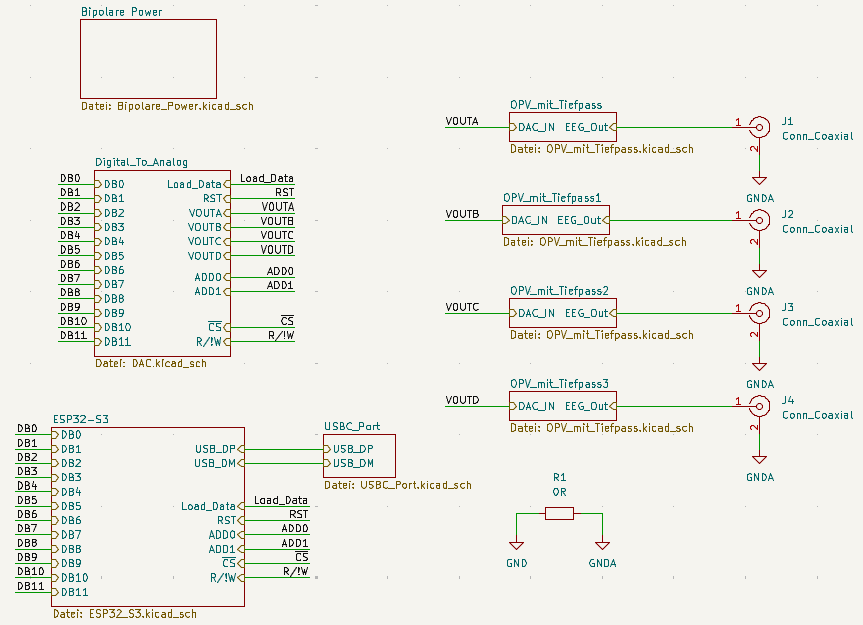
\includegraphics[width=0.8\textwidth]{bilder/Platine_gesamt.png}
    \caption{Gesamtübersicht der Platine}
    \label{fig:gesamtuebersicht}
\end{figure}
Die Platine ist in mehrere Funktionsblöcke unterteilt, die jeweils für spezifische Aufgaben zuständig sind. Diese Blöcke sind:
\begin{itemize}
    \item \textbf{Mikrocontroller-Block:} Enthält den ESP32-S3 16R8, der die Signalverarbeitung und die Weboberfläche steuert.
    \item \textbf{DAC-Block:} Beinhaltet den DAC8412FPZ, der die digitalen Signale in analoge Signale umwandelt.
    \item \textbf{Operationsverstärker-Block:} Besteht aus dem TL071CDR, der als aktiver Tiefpassfilter fungiert.
    \item \textbf{Spannungsversorgungsblock:} Umfasst die LDOs, den DCDC Wandler und die beiden Shunt Spannungsreferenzen zur Bereitstellung der benötigten Spannungen und Referenzen.
    \item \textbf{USB-Block:} Dient der Stromversorgung der Platine über eine USB-Schnittstelle.
\end{itemize}

\subsection{Mikrocontroller-Block}
\begin{figure}[H]
    \centering
    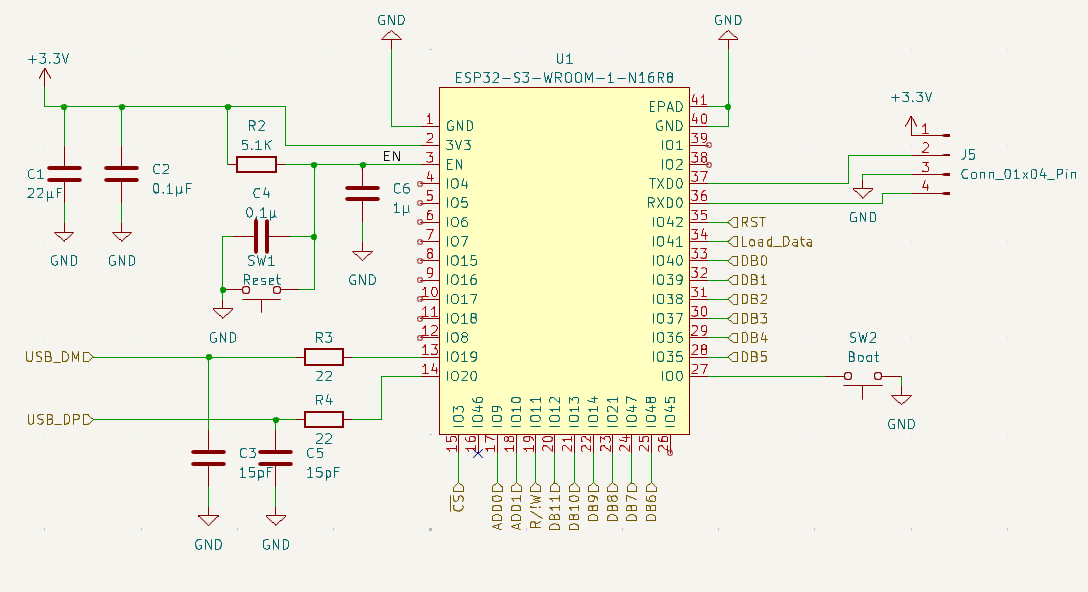
\includegraphics[width=0.8\textwidth]{bilder/Mikrocontroller_Block.png}
    \caption{Mikrocontroller-Block der Platine}
    \label{fig:mikrocontroller_block}
\end{figure}

Der Mikrocontroller-Block enthält den ESP32-S3 16R8, der die zentrale Steuereinheit der Platine darstellt. Er ist für die Signalverarbeitung, die Bereitstellung der Weboberfläche und Speicherung der EEG-Simulationsdaten verantwortlich. Der Mikrocontroller kommuniziert über eine parallele Schnittstelle mit dem \gls{dac} und steuert dessen Ausgänge.\\
Die Programmierung des Mikrocontrollers erfolgt in C++ unter Verwendung der Arduino-IDE mit PlatformIO. 

\subsection{DAC-Block}
\begin{figure}[H]
    \centering
    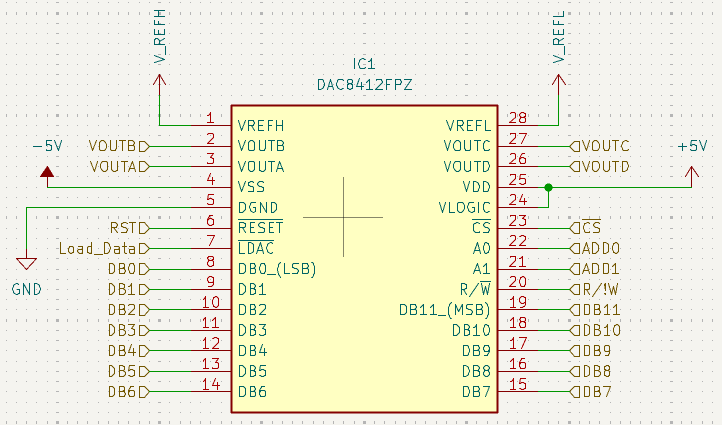
\includegraphics[width=0.8\textwidth]{bilder/DAC.png}
    \caption{DAC-Block der Platine}
    \label{fig:dac_block}
\end{figure}

Der DAC-Block enthält den DAC8412FPZ mit seiner speziellen Beschaltung.
Der \gls{dac} wandelt die digitalen Signale des Mikrocontrollers in analoge Signale umwandelt. Hierbei werden die Signal mit einer Parallelen-Schnittstelle übertragen, die es durch gleichzeitiges bereitstellen der einzelnen Digitalen Bits, ermöglichst eine hohe Datenrate bereitzustellen. Der DAC8412FPZ bietet eine Auflösung von 12 Bit und vier unabhängige Ausgänge, die jeweils für die Ausgabe eines EEG-Signals verwendet werden können.\\
Die Signale werden vom Mikrocontroller bereitgestellt und über die parallele Schnittstelle an den DAC übertragen. Der DAC wandelt diese Signale in analoge Spannungen um, die dann weiterverarbeitet werden.\\

\subsection{Operationsverstärker-Block}
\begin{figure}[H]
    \centering
    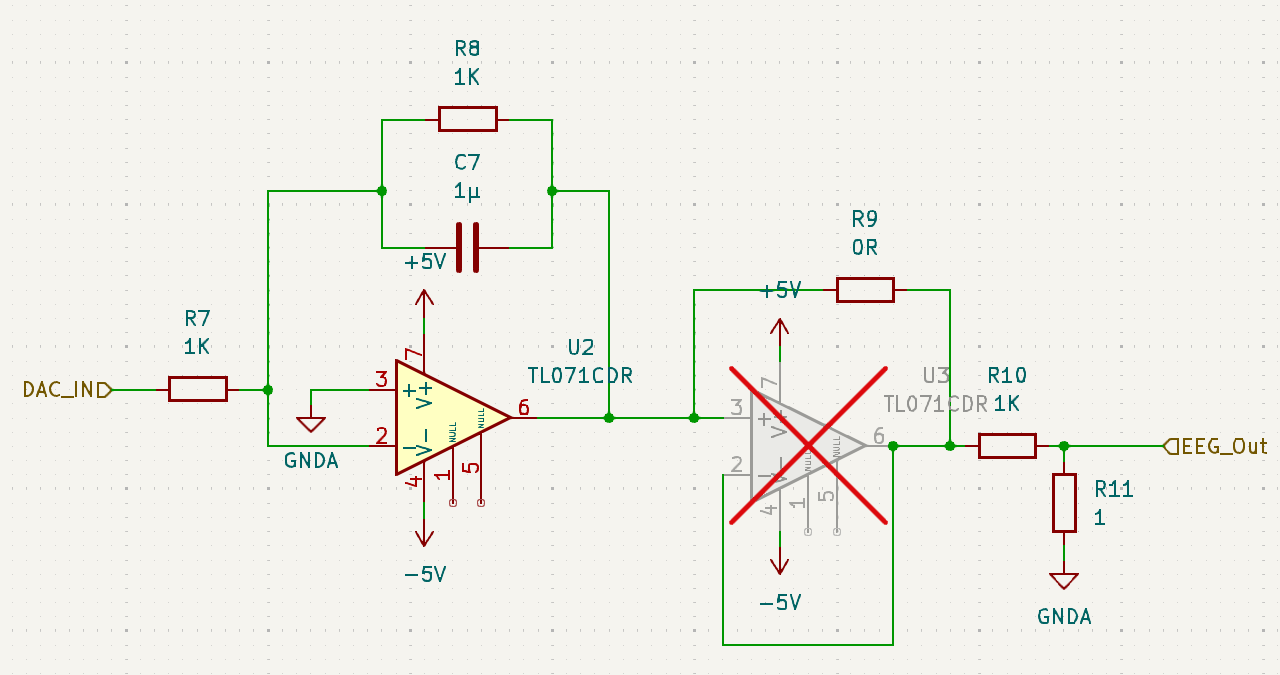
\includegraphics[width=0.8\textwidth]{bilder/Operationsverstaerker_Block.png}
    \caption{Operationsverstärker-Block der Platine}
    \label{fig:operationsverstaerker_block}
\end{figure}

Der Operationsverstärker-Block enthält den TL071CDR, der als aktiver Tiefpassfilter fungiert. Dieser glättet die analogen Signale des \gls{dac} und reduziert hochfrequentes Rauschen. Der Operationsverstärker ist so konfiguriert, dass er eine Verstärkung von 1 bietet, um die Ausgangsspannungen im Millivolt-Bereich zu halten.\\
Im weiter inst noch möglich einen weiterer Operationsverstärker zu verbauen der als Spannungsfolger fungieren kann, um die Ausgangsimpedanz zu reduzieren und die Signalqualität zu verbessern. Standardmäßig ist dieser nicht verbaut und mit einem Jumper überbrückt. 

\subsection{Spannungsversorgung}
\begin{figure}[H]
    \centering
    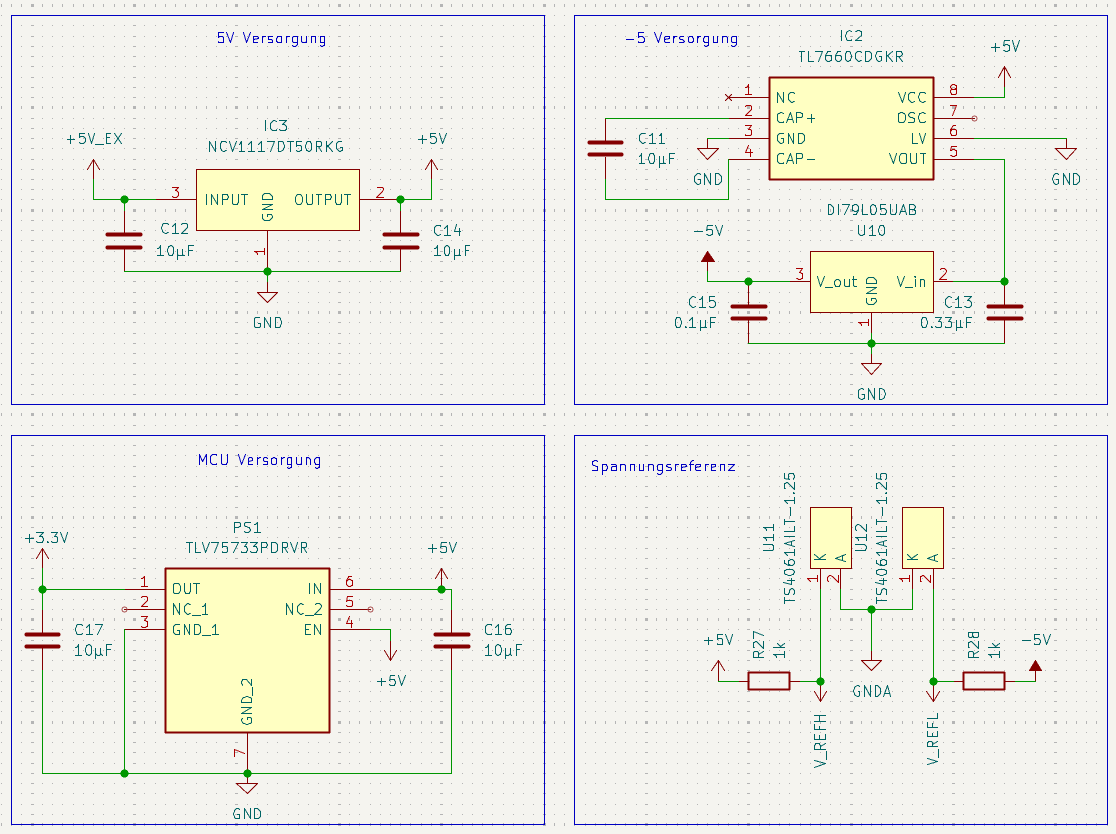
\includegraphics[width=0.8\textwidth]{bilder/Bipolar_Power.png}
    \caption{Spannungsversorgungsblock der Platine}
    \label{fig:spannungsversorgung}
\end{figure}
Die Spannungsversorgung der Platine erfolgt über eine USB-Schnittstelle, die 5V bereitstellt. 
Diese wird durch den LDO NCV1117DT50RKG auf 5V für den DAC und den Operationsverstärker geglättet.\\
Für die Versorgung des Mikrocontrollers ist der TLV75733PDRVR zuständig, der eine stabile 3.3V Versorgungsspannung liefert.
Da der \gls{dac} DAC8412FPZ eine symmetrische Versorgungsspannung von \pm 5V benötigt, wird ein invertierter DCDC Wandler LT3580EDD verwendet, der aus der 5V Versorgungsspannung eine negative Spannung von -5V erzeugt. Die wird zusätzlich auch für die Versorgung der Operationsverstärker genutzt.\\
Da der \gls{dac} eine Referenzspannung benötigt, wird eine stabile \pm 1.25V Referenzspannung durch zwei TS4061AILT-1.25 bereitgestellt. 

\subsection{USB-Block}
\begin{figure}[H]
    \centering
    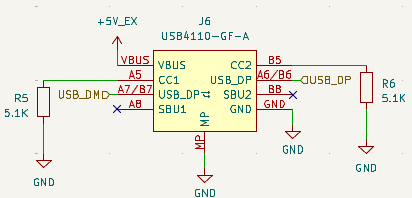
\includegraphics[width=0.8\textwidth]{bilder/USBC_Port.png}
    \caption{USB-Block der Platine}
    \label{fig:usb_block}
\end{figure}
Der USB-Block dient der Stromversorgung der Platine über eine USB-Schnittstelle. Er enthält die notwendigen Schaltungen, um die 5V Versorgungsspannung der USB-Schnittstelle einzustellen und die Kommunikation mit dem Mikrocontroller zu ermöglichen.\\